\documentclass[a4paper]{article}

% natbib
\usepackage[numbers,sort]{natbib}

\usepackage{mysimpletemplatewn}
\usepackage[utf8]{inputenc} %%% to support copy and paste with accents for french stuff
\usepackage[T1]{fontenc} %%%key to get copy and paste for the code!
\usepackage{times}
\usepackage[french]{babel}
\usepackage[scaled=0.85]{helvet}
\usepackage{graphicx}
\usepackage{ifthen}
\usepackage{xspace}
\usepackage{alltt}
\usepackage{latexsym}
\usepackage{url}
\usepackage{amsmath,amssymb,amsfonts}
\usepackage{stmaryrd}
\usepackage{algorithmic}
\usepackage{textcomp}
\usepackage{xcolor}
\usepackage{enumerate}
% \usepackage{cite}
\usepackage[pdftex,colorlinks=true,pdfstartview=FitV,linkcolor=blue,citecolor=blue,urlcolor=blue]{hyperref}
\usepackage{multirow}
\usepackage{listings}
\usepackage{color}
\usepackage{subcaption}

\usepackage{pgfgantt}

\usepackage{bibentry}
\nobibliography*


\newboolean{showcomments}
\setboolean{showcomments}{true}
\ifthenelse{\boolean{showcomments}}
  {\newcommand{\bnote}[2]{
	\fbox{\bfseries\sffamily\scriptsize#1}
    {\sf\small$\blacktriangleright$\textit{#2}$\blacktriangleleft$}
    % \marginpar{\fbox{\bfseries\sffamily#1}}
   }
   \newcommand{\paragraphDesc}[2]{
    \textcolor{#1}{#2}
   }
   
  }
  {\newcommand{\bnote}[2]{}
   \newcommand{\cvsversion}{}
   \newcommand{\paragraphDesc}[2]{}
  }

\newcommand{\here}{\bnote{***}{CONTINUE HERE}}
\newcommand{\nb}[1]{\bnote{NB}{#1}}

\newcommand{\fix}[1]{\bnote{FIX}{#1}}
%%%% add your own macros 


\newcommand{\sd}[1]{\bnote{Stef}{\textcolor{orange}{#1}}}
\newcommand{\an}[1]{\bnote{Anne}{\textcolor{green}{#1}}}
\newcommand{\bv}[1]{\bnote{Benoit}{\textcolor{blue}{#1}}}
\newcommand{\nic}[1]{\bnote{Nic}{\textcolor{red}{#1}}}

\newcommand{\todo}[1]{\bnote{TODO}{#1}}

\graphicspath{{figures/}}
%%% 


\newcommand{\figref}[1]{Figure~\ref{fig:#1}}
\newcommand{\figlabel}[1]{\label{fig:#1}}
\newcommand{\tabref}[1]{Table~\ref{tab:#1}}
\newcommand{\layout}[1]{#1}
\newcommand{\commented}[1]{}
\newcommand{\secref}[1]{Section~\ref{sec:#1}}
\newcommand{\seclabel}[1]{\label{sec:#1}}

%\newcommand{\ct}[1]{\textsf{#1}}
\newcommand{\stCode}[1]{\textsf{#1}}
\newcommand{\stMethod}[1]{\textsf{#1}}
\newcommand{\sep}{\texttt{>>}\xspace}
\newcommand{\stAssoc}{\texttt{->}\xspace}

\newcommand{\stBar}{$\mid$}
\newcommand{\stSelector}{$\gg$}
\newcommand{\ret}{\^{}}
\newcommand{\msup}{$>$}
%\newcommand{\ret}{$\uparrow$\xspace}

\newcommand{\myparagraph}[1]{\noindent\textbf{#1.}}
\newcommand{\eg}{\emph{e.g.}\xspace}
\newcommand{\ie}{\emph{i.e.}\xspace}
\newcommand{\etal}{\emph{et al.,}\xspace}
\newcommand{\ct}[1]{{\textsf{#1}}\xspace}
\newcommand{\etc}[1]{\textit{etc.}}



\newcommand{\defaultScale}{0.55}
\newcommand{\pic}[3]{
   \begin{figure}[h]
   \begin{center}
   \includegraphics[scale=\defaultScale]{#1}
   \caption{#2}
   \label{#3}
   \end{center}
   \end{figure}
}


\newcommand{\twocolumnpic}[3]{
  \begin{figure*}[!ht]
  \begin{center}
  \includegraphics[scale=\defaultScale]{#1}
  \caption{#2}
  \label{#3}
  \end{center}
  \end{figure*}
}

\newcommand{\picw}[3]{
  \begin{figure}[htbp]
  \begin{center}
  \includegraphics[width=\columnwidth]{#1}
  \caption{#2}
  \label{#3}
  \end{center}
  \end{figure}
}


\newcommand{\infe}{$<$}
\newcommand{\supe}{$\rightarrow$\xspace}
\newcommand{\di}{$\gg$\xspace}
\newcommand{\adhoc}{\textit{ad-hoc}\xspace}

\usepackage{url}            
\makeatletter
\def\url@leostyle{%
  \@ifundefined{selectfont}{\def\UrlFont{\sf}}{\def\UrlFont{\small\sffamily}}}
\makeatother
% Now actually use the newly defined style.
\urlstyle{leo}

\definecolor{codegreen}{rgb}{0,0.6,0}
\definecolor{codegray}{rgb}{0.5,0.5,0.5}
\definecolor{codepurple}{rgb}{0.58,0,0.82}
\definecolor{backcolour}{rgb}{0.95,0.95,0.92}

\lstdefinestyle{mystyle}{
    backgroundcolor=\color{backcolour},
    commentstyle=\color{codegreen},
    keywordstyle=\color{magenta},
    numberstyle=\tiny\color{codegray},
    stringstyle=\color{codepurple},
    basicstyle=\footnotesize,
    breakatwhitespace=false,
    breaklines=true,
    captionpos=b,
    keepspaces=true,
    numbers=left,
    numbersep=5pt,
    showspaces=false,
    showstringspaces=false,
    showtabs=false,
    tabsize=2
}

\lstset{style=mystyle}


\title{CST --Analyse multi-facettes et opérationnelle pour la transformation des systemes d’information}
\author{ HOUEKPETODJI Mahugnon Honoré}

\begin{document}

\institution{}

\date{\today}

\maketitle

% \begin{abstract}
% The abstract text goes here.
% \end{abstract}

\section{Description du sujet de la thèse}
% 0.5 (1/2) pages
CIM est une SAS au capital social de 200k détenu a 100% par DL Software. CIM est´editeur, int´egrateur, h´ebergeur et infog´ereur de solutions pour l’assurance de personnes
en sant´e, pr´evoyance. Elle offre une expertise Sant´e et Pr´evoyance acquise apr`es
plus de 30 ans aupr`es de ses clients. CIM est h´ebergeur de ses solutions pour 90% de
ses clients et plus de 1000 utilisateurs. Toutes les th´ematiques d’infrastructure et de
surveillance des flux sont int´egr´ees `a cette offre. CIM est propri´etaire de ses infrastructures
serveurs, tous les ´el´ements actifs des syst`emes et tous les ´el´ements de stockage
sont achet´es par CIM, g´er´es et supervis´es par les ´equipes de CIM. Aucun sous-traitant
n’intervient dans les op´erations quotidiennes d’h´ebergement, d’exploitation des solutions
et des donn´ees h´eberg´ees.
\section{Etat de l'art}
\label{sec:stateOfTheArt}
% 1 pages

% \secref{literatureMigrationConstraint} présente la contrainte de migration trouvée dans la littérature.
La~\secref{migrationTechnique} présente les techniques utilisées pour migrer une application.
\secref{position}, nous décrivons les méta-modèles d'interface graphiques trouvés dans la littérature.

\subsection{Stratégie de migration existantes}
\label{sec:migrationTechnique}

Pour définir une stratégie de migration, nous avons identifié des travaux de recherche liés à la migration des applications.
Certaines des approches proposées n'effectuent pas une migration complète, mais seulement en partie.
Toutes les approches utilisent des techniques de rétroingénierie.
De plus, il existe de nombreuses publications traitant de la migration de langage de programmation.
Nous ne les considérons cependant pas si elles ne discutent pas explicitement de la migration d'interfaces graphiques.
C'est le cas, par exemple, du travail de \citet{Bran10a} qui fait état d'une importante migration de Delphi vers C\#.

Nous avons identifié trois techniques pour créer une représentation d'interfaces graphiques :
statique, dynamique ou hybride.

\textbf{Statique}. La stratégie statique consiste à analyser le code source et à en extraire des informations. 
Le code de l'application analysée n'est donc pas exécuté.

\citet{Clou16a} analyse directement les fichiers HTML, CSS et JavaScript.
L'analyse construit un arbre syntaxique du code source du site web 
  et extrait les widgets des fichiers HTML.
Le travail consiste principalement à identifier les liens entre les éléments du programme source (classes JavaScript, balises HTML, \etc). 
Le travail présenté n'aborde pas la migration complète de l'interface graphique.

\citet{Silv10a, Lell16a} et \citet{Stai07a} ont utilisé des outils qui analysent
  le code source des applications de bureau.
Les outils recherchent la création des widgets dans le code source,
  puis ils analysent les méthodes qui invoquent ou sont invoquées par les widgets pour
  identifier les relations entre les widgets et leurs propriétés visuelles.

\citet{Sanc14a} et \citet{Garce17b} ont développé des approches pour extraire l'interface graphique des applications Oracle Forms.
Avec ce framework, les développeurs définissent les interfaces dans des fichiers externes où la position de chaque widget est spécifiée.
Leur approche consiste à créer la hiérarchie des widgets à partir de leur position.
Cependant, ces études de cas sont simples et ne comportent que peu de formulaires ou de textes.
La mise en page est également simple car tous les éléments sont affichés les uns en dessous des autres.

% La stratégie statique permet d'analyser une application sans avoir à l'exécuter ni même à la compiler.
Outre le problème classique de montrer les résultats de toutes les éxecutions possible plutôt 
  que celui obtenu lors de l'execution du programme, 
  une autre limitation apparaît par exemple, avec une application client/serveur, 
    quand une partie de l'interface graphique dépend du résultat d'une requête à un serveur.

\textbf{Dynamique}. La stratégie dynamique consiste à analyser les interfaces graphiques d'une application en cours d'exécution.
Elle explore les états de l'application en effectuant toutes les actions possibles sur l'interface graphique du logiciel
  et extrait les widgets et leurs informations.

\citet{Memo03b, Sami07a, Shah11b} et \citet{Morg11a} ont développé des outils qui mettent en œuvre une stratégie dynamique.
Cependant, les solutions proposées ne sont disponibles que pour les applications de bureau et non pour les applications web.

Bien que l'analyse dynamique recueille des informations détaillées sur toutes les fenêtres d'une application,
  l'exécution automatique d'une application pour capturer méthodiquement tous ses écrans peut être une tâche difficile en fonction de la technologie utilisée.
De plus, si une requête serveur est utilisée pour construire une des interfaces graphiques, l'analyse dynamique ne détecte pas cette information qui peut être essentielle pour la représentation complète des interfaces.

\textbf{Hybrid}. La stratégie hybride tente de combiner les avantages des analyses statiques et dynamiques.

\citet{Gott16a} a utilisé une stratégie hybride pour analyser des applications Java.
Ils créent d'abord un modèle à partir d'une analyse statique du code source.
L'analyse statique trouve les widgets et attributs d'une interface graphique et leurs structures.
Ensuite, l'analyse dynamique exécute toutes les actions possibles liées à un widget et analyse si
  une modification se produit sur l'interface.

Malgré l'utilisation de l'analyse statique et dynamique, la stratégie hybride ne résout pas le problème de requête inhérent aux applications client/serveur.
Il a également les mêmes problèmes que l'analyse dynamique de l'exécution automatique d'une application et de la capture de ses écrans.

\citet{Fleu07b} et \citet{Garce17b} ont travaillé sur la migration complète de logiciels.
Ils ont développé un outil qui effectue la migration de façon semi-automatique.
Pour ce faire, ils ont utilisé le procédé du fer à cheval (\citet{Kazm98a}). 
La migration est divisée en quatre étapes :

\begin{enumerate}
\def\labelenumi{\arabic{enumi}.}
    \item Génération du modèle de l'application originale.
    \item Transformation de ce modèle en modèle pivot.
Cela comprend les structures de données, les actions et algorithmes, l'interface utilisateur et la navigation.
    \item
Transformation du modèle pivot en modèle du langage cible.
    \item
Génération du code source dans le langage cible.
\end{enumerate}

\noindent\hfil\rule{8cm}{0.5pt}\hfil

Aucun des auteurs n'a envisagé la migration des interfaces graphiques du web vers des interfaces graphiques du web.
De plus, aucun n'avait la contrainte de garder une mise en page similaire sauf \citet{Sanc14a} ; 
  cependant, ils travaillaient sur des applications Oracle Forms qui ont des interfaces très différentes de celles que l'on retrouve dans le web.
Par conséquent, leur travail n'est pas directement applicable à notre étude de cas.

\noindent\hfil\rule{8cm}{0.5pt}\hfil

\subsection{Représentation de l'interface utilisateur}
\label{sec:position}

Dans la section précédente, de nombreuses représentations abstraites d'interfaces graphiques sont utilisées.
L'utilisation de représentation abstraite, souvent mise en place grâce à des méta-modèles, permet aux auteurs
  de manipuler les concepts les plus importants de leurs domaines et de réutiliser ces modèles pour différents travaux, \eg génération, migration, analyse, \etc.
Nous avons examiné les représentations proposées et les avons comparées.
Nous présentons maintenant les deux méta-modèles d'interface graphique définis par l'OMG. 
Le "Knowledge Discovery Metamodel" (KDM) permet de représenter tout type d'application.
L'"Interaction Flow Modeling Language" (IFML) est spécialisé dans les applications avec interface graphique.
La~\secref{stateMetaUI} présente d'autres représentations décrites dans la littérature et les compare à celles de l'OMG.

\subsubsection{Les standards de l'OMG}
\label{sec:omg}

L'OMG définit la norme KDM pour aider l'évolution des logiciels.
La norme définit un méta-modèle pour représenter un logiciel à un haut niveau d'abstraction.
Il inclut un module d'interface graphique qui représente les composants et le comportement d'une interface graphique.

\begin{figure}
    \centering
    \begin{minipage}{.5\textwidth}
      \centering
      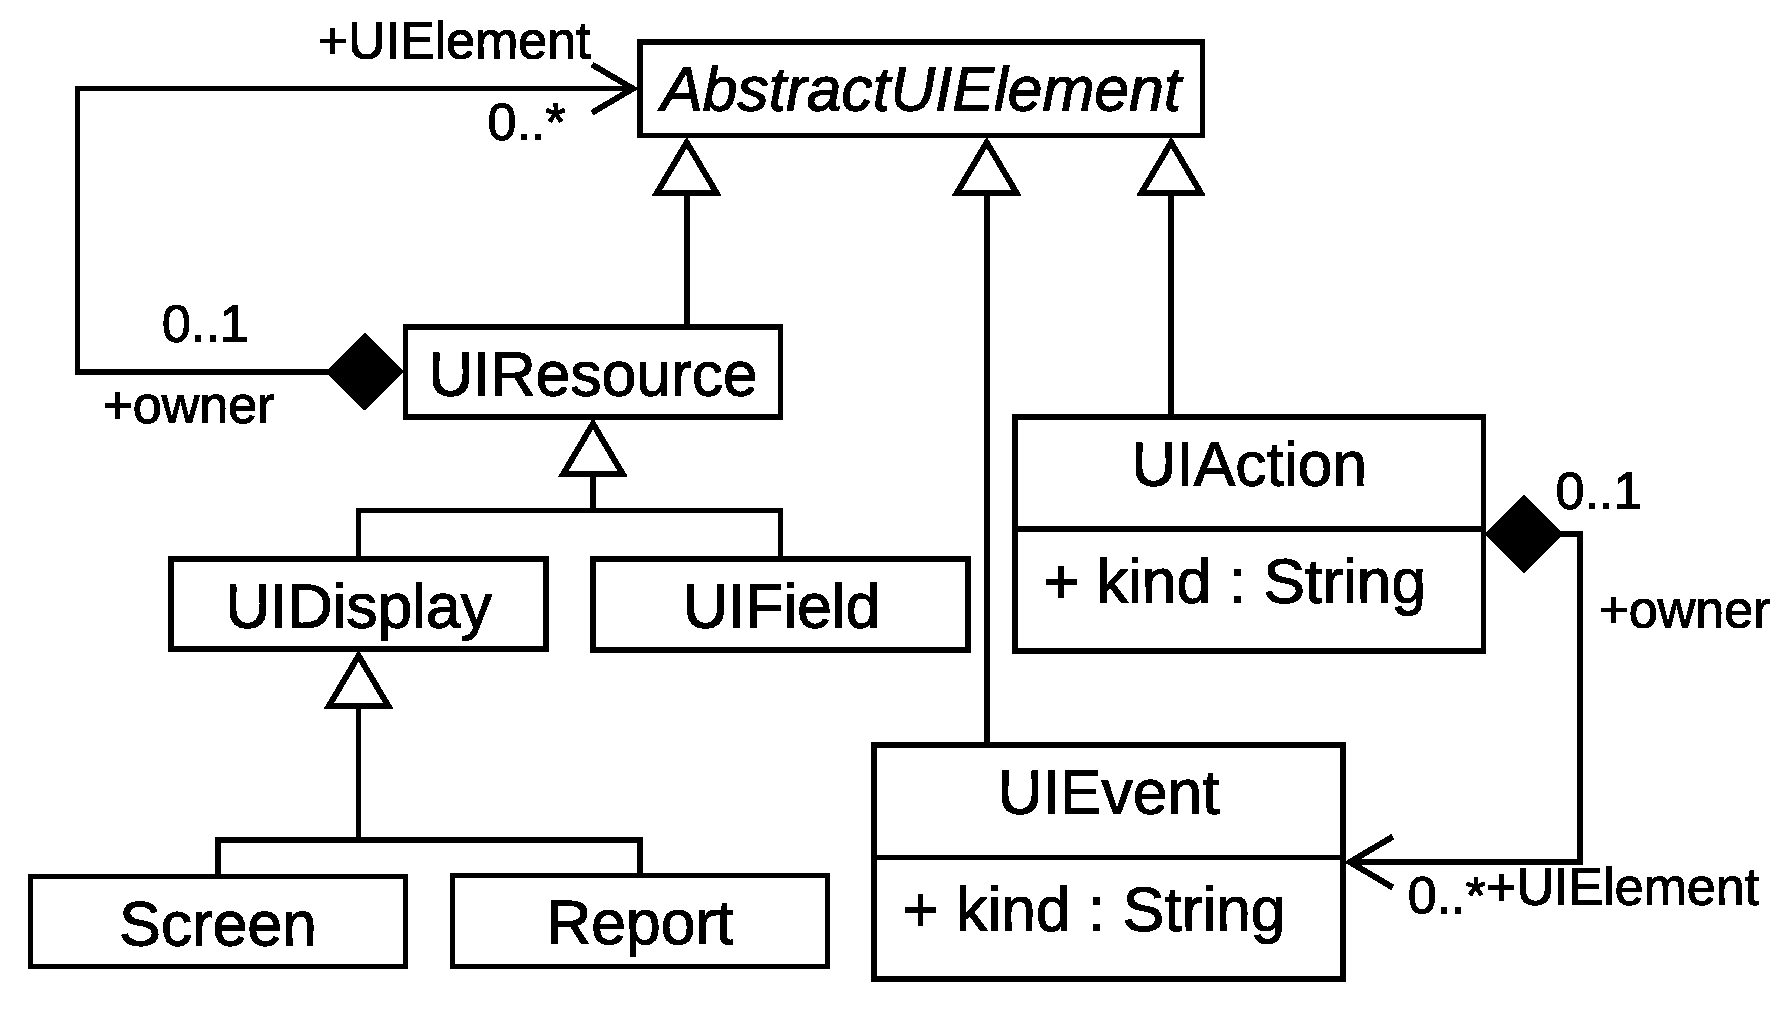
\includegraphics[width=.9\linewidth]{kdm}
      \captionof{figure}{KDM - Diagramme de classes UIResources}
      \label{fig:kdm}
    \end{minipage}%
    \begin{minipage}{.5\textwidth}
      \centering
      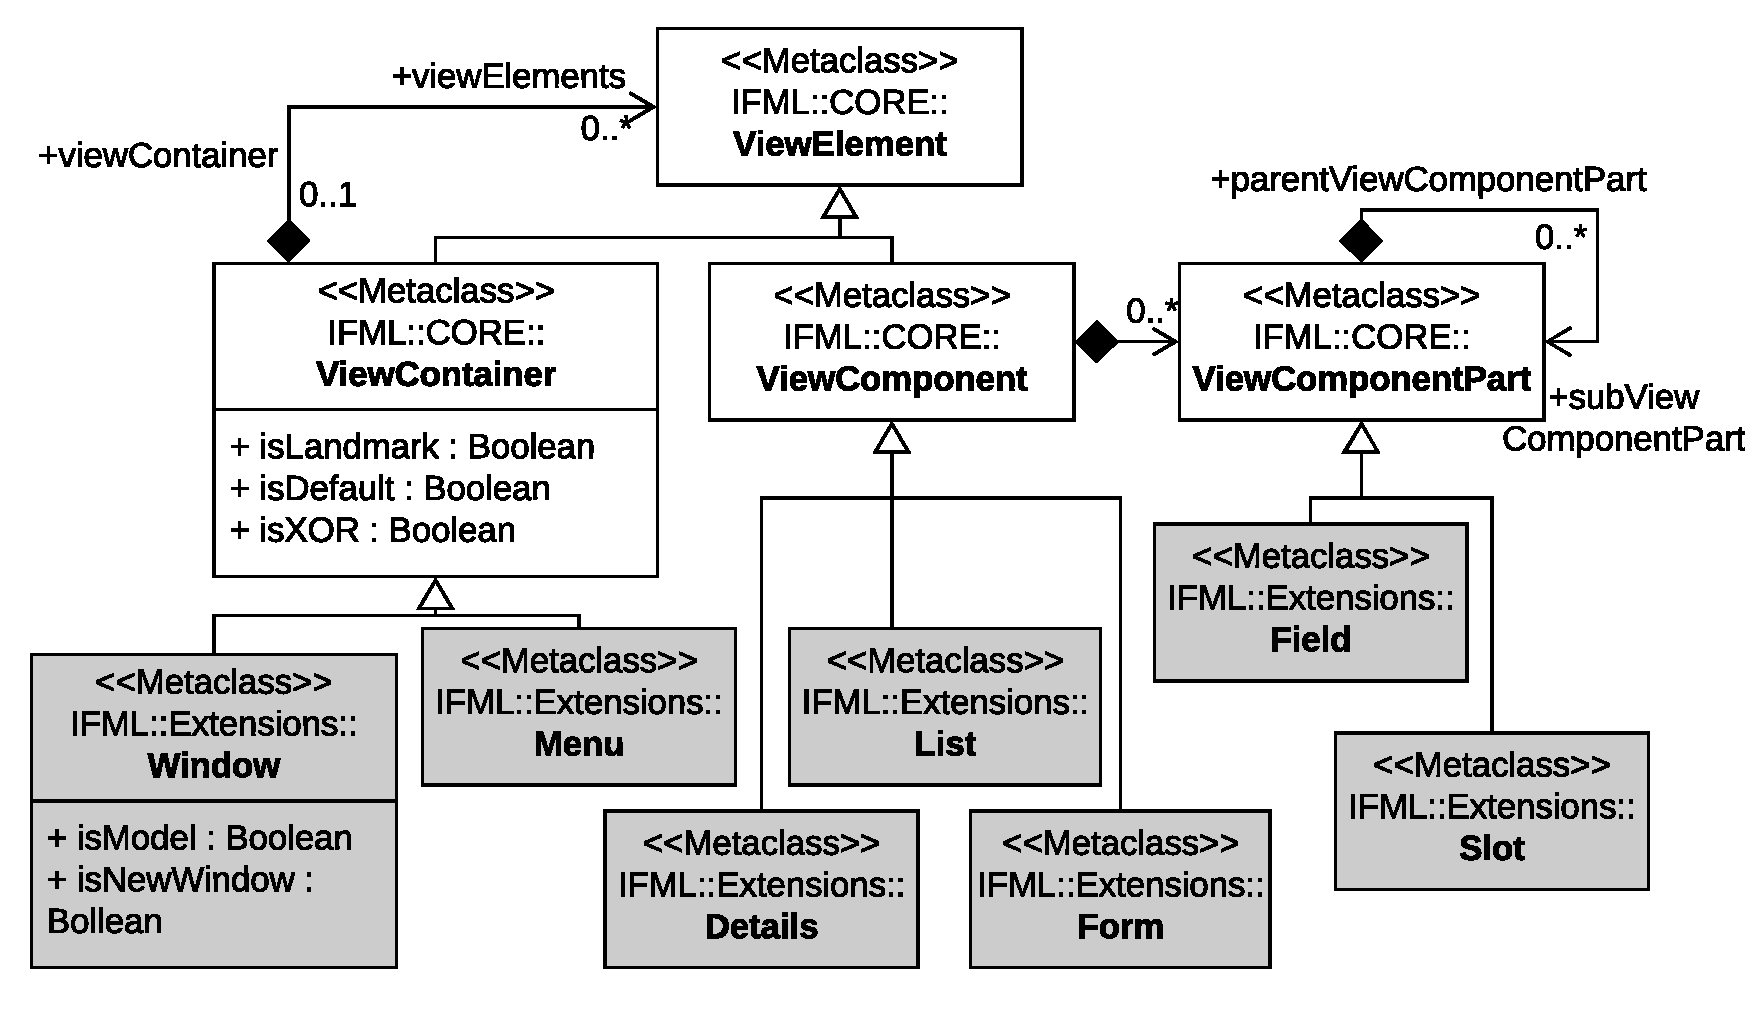
\includegraphics[width=.9\linewidth]{ifml}
      \captionof{figure}{IFML - View Elements}
      \label{fig:ifml}
    \end{minipage}
\end{figure}

La \figref{kdm} représente les entités principales de la partie de l'interface utilisateur appelée diagramme de classes UIResources.
L'entité principale est UIResource.
Elle peut être affinée comme UIDisplay ou UIField.
UIDisplay correspond au support physique sur lequel l'interface sera affichée, \eg un écran d'ordinateur, un rapport imprimé, \etc.
UIField correspond à un widget d'une interface graphique, \eg un formulaire, un champ texte, un panneau, \etc.
La composition entre UIResource et AbstractUIElement est utilisée pour définir le DOM (Document Object Model).
Chaque UIResource peut en contenir un autre pour représenter un widget qui contient un autre widget.

Un UIResource peut avoir, par composition, une UIAction pour représenter le comportement de l'interface graphique.

Le but de IFML \citep{Bram14a} est de fournir des outils pour décrire la partie visuelle d'une application,
  avec les composants et les conteneurs, l'état des composants,
  la logique de l'application et le lien entre les données et l'interface graphique.


La \figref{ifml} représente le méta-modèle de la partie visuelle d'une application.
Les éléments visibles de l'interface graphique sont appelés ViewElement.
Un ViewElement peut être affiné comme un ViewContainer ou un ViewComponent. 

Un ViewContainer représente un conteneur d'autres ViewContainers ou ViewComponents.
Par exemple, cela peut être une fenêtre, une page HTML, un panneau \etc..
La composition entre ViewContainer et ViewElement est utilisée pour définir le DOM.

Un ViewComponent correspond à un widget qui affiche son contenu, par exemple un formulaire, un tableau, une galerie d'images, \etc.
Il peut être lié à plusieurs ViewComponentPart.
Un ViewComponentPart représente un élément d'un ViewComponent.
Par exemple,
  un champ de saisie dans un formulaire,
  un texte qui est affiché à l'intérieur d'un tableau,
  ou une image d'une galerie.

\subsubsection{méta-modèles GUI dans la littérature}
\label{sec:stateMetaUI}

D'autres méta-modèles d'interfaces graphiques ont été proposés dans la littérature.
Nous les comparons aux normes de l'OMG.

Tous les méta-modèles utilisent le patron de conception Composite pour représenter le DOM d'une interface graphique et
  définissent une entité correspondant à UIResource pour représenter un élément graphique d'une interface.

\citet{Gott16a} et \citet{Sanc14a} ont proposé un méta-modèle inspiré du modèle KDM.
Le méta-modèle est composé des entités principales définies par KDM.
Les deux auteurs ont ajouté l'entité Attribute au méta-modèle.
Ils définissent également différents types de widgets tels que Button, Label, Panel, \etc.

\citet{Fleu07b} ne décrivaient pas explicitement le méta-modèle de l'interface graphique,
  mais nous avons extrait des informations de leur modèle de navigation.
Ils ont au moins deux éléments dans leur modèle d'interface graphique qui représentent une Window
    et un GraphicElement.
La Windows correspond à l'entité Display du modèle KDM.
Et parce que le GraphicElement et le Window ne sont pas liés,
    on peut supposer que le GraphicElement est une source UIRessource.
Le GraphicElement a un Event.

\citet{Morg11a} ont utilisé un méta-modèle d'interface graphique mais ne l'ont pas décrit.
Nous savons seulement que l'interface graphique est représentée sous la forme d'un arbre similaire au DOM.

Le méta-modèle UI de \citet{Garce17b} diffère beaucoup des précédents.
Il y a les attributs, les événements et la page mais la notion de widget est présente comme un champ qui affiche les données d'une table.
Ils ont également utilisé une entité Event pour représenter l'interaction de l'utilisateur avec l'interface utilisateur.
L'entité Event correspond aux entités Action et Event du modèle KDM.

\citet{Memo03b} ont représenté une interface graphique avec seulement deux entités.
Une fenêtre de l'interface graphique qui est composée d'un ensemble de widgets qui peuvent avoir des attributs.
Représenter les DOM n'était pas dans le cadre de leur travail.
Il n'est pas possible de le représenter avec leur méta-modèle.

\citet{Sami07a} ont travaillé sur la migration des applications Java-Swing vers des applications web Ajax.
Ils ont créé un méta-modèle pour représenter l'interface graphique de l'application originale.
Ce méta-modèle est stocké dans un fichier XUL (langage d'interface graphique basé sur XML) et représente
  les widgets avec leurs attributs et la mise en page.
Ces widgets appartiennent à une Window et
  peut déclencher des événements lorsqu'une action est effectuée sur l'interface graphique.
L'action et l'événement correspondent aux entités Action et Event du modèle KDM.
Le format XUL a été abandonné.

\citet{Shah11b} ont utilisé une architecture arborescente pour représenter les interfaces graphiques.
Cela leur permet de modéliser le DOM.
La racine de l'arbre est un Frame.
Il correspond à l'entité UIDisplay.
La racine contient les composants avec leurs attributs.

\citet{Joor12a} ont représenté une interface graphique avec un ensemble d'éléments graphiques.
Ces éléments correspondent à la définition d'un UIField.
Pour chaque élément de l'interface, l'outil des auteurs détecte de multiples attributs et actions.

\citet{Memo07a} utilise un modèle d'interface graphique pour représenter l'état d'une application.
Un état est défini à partir des widgets de l'interface graphique et leurs propriétés.

\citet{Mesb12a} n'ont pas présenté directement leur méta-modèle pour les interfaces graphiques.
Cependant, ils expliquent utiliser une représentation arborescente pour analyser différentes pages web.
Ils ont également utilisé la notion d'événements qui peuvent être déclenchés.
Ils ont utilisé différentes instances de leur méta-modèle d'interface graphique pour représenter les pages web de l'application.
Ces instances peuvent être comparées à plusieurs entités UIDisplay.

Tous les auteurs ont utilisé la notion de widget qui représente une entité visuelle de l'interface graphique.
La plupart d'entre eux ont une entité attribut qui représente une caractéristique d'un widget.
Enfin, les liens de navigation sont représentés par une entité d'action.

\section{Avancées actuelles}
% 3 pages

Des premiers travaux ont été menés sur le projet de migration.
La~\secref{context} présente le travail d'analyse que nous avons mené afin de comprendre plus précisément les éléments concernés par la migration du \textit{front-end} d'une application.
La~\secref{approche} présente l'approche que nous utilisons ainsi que le méta-modèle d'interface graphique qu'elle utilise.
La~\secref{resultats} présente les premiers résultats que nous avons obtenus et publiés.

\subsection{Context}
\label{sec:context}

Dans la~\secref{comparisonGwtAngular} nous décrivons les principales différences entre les applications GWT et Angular.
Dans la~\secref{guiDecomposition} nous présentons une catégorisation du code source du front-end.

\subsubsection{Comparison de GWT et Angular}
\label{sec:comparisonGwtAngular}

Dans ce projet, la langue source et la langue cible imposent deux schémas d'organisation différents. 
Leurs différences sont syntaxiques et sémantiques.

GWT est un framework qui permet aux développeurs d'écrire une application web en Java.
Le code GUI est compilé en code HTML, CSS et JavaScript.
Angular est un framework d'application web qui
  permet aux développeurs d'écrire une application web avec le langage TypeScript.
Il est utilisé pour créer des Single-Page Applications\footnote{Les Single-Page Applications (SPA) sont des applications web qui chargent une seule page HTML et mettent à jour dynamiquement cette page lorsque l'utilisateur interagit avec l'application.}

Les trois principales différences entre 
  les applications GWT et Angular sont : la définition des pages web, leur style et les fichiers de configuration.
Avant d'expliquer ces trois différences, nous notons une similitude majeure : 
  les applications GWT et Angular ont toutes deux un fichier CSS principal pour définir l'aspect visuel général de l'application.

\begin{itemize}
\item \textbf{Définition de page web.} 
Dans le framework GWT, un seul fichier Java est nécessaire pour définir une page web.
Le fichier Java (GWT) comprend les principaux composants graphiques (widgets) de la page web,
  leurs positions et leurs organisations hiérarchiques.
Dans le cas d'un widget actionnable (comme un bouton), l'action est implémentée dans le même fichier.
Dans Angular, il existe une hiérarchie de fichiers pour chaque page web.
Chaque page web est considérée comme un sous-projet indépendant des autres.
Un sous-projet contient deux fichiers :
  un fichier HTML, contenant les widgets de la page web et leurs organisations ; 
  et un fichier TypeScript, contenant le code à exécuter lorsqu'une action est exécutée. 

\item \textbf{Aspect visuel}
L'aspect visuel d'une page web comprend la couleur ou les dimensions spécifiques des éléments affichés.
Dans le cas de GWT, l'aspect visuel spécifique est défini dans le fichier Java du fichier de définition de la page web.
Dans Angular, il existe un fichier CSS distinct optionnel.

\begin{figure}[htbp]
  \centering
  \begin{lstlisting}
<application name="CORE-Incubator">
	<module name="KITCHENSINK">
    <phase codePhase="KITCHENSINK_HOME" 
      className="fr.bl.client.kitchensink.PhaseHomeKitchenSink" 
      title="Home"/>
  </module>
</application>
  \end{lstlisting}
  \caption{Exemple d'un fichier de configuration GWT en XML}
  \label{fig:xmlExample}
\end{figure}


\item \textbf{Fichiers de configuration}
Pour les fichiers de configuration, GWT utilise un fichier XML qui définit les
  liens entre un fichier Java, une page web et l'URL de la page web.
La~\figref{xmlExample} présente un extrait du fichier XML d'une application de Berger-Levrault.
La balise application est la balise racine du fichier.
Elle définit le nom de l'application GWT.
% Une application consiste en plusieurs \tagc{module}s et un \tagc{module} en
% multiple \tagc{phase}.
%\tagc{Module} définit un groupe de code GWT qui est utilisé dans
% de projets GWT multiples.
La balise phase (ligne 3) définit une page web de l'application GWT : Le titre de la page web est "Home" ;
  elle est définie par la classe Java \texttt{PhaseHomeHomeKitchenSink} (dans le paquetage \texttt{fr.bl.client.kitchensink}) ; et
  l'URL pour accéder à la page web est \texttt{adresseduserveur.com/KITCHENSINK\_HOME}.
Pour Angular, il existe deux fichiers de configuration : \emph{module} qui définit les composants de l'application, \eg pages web, services distants et composant graphiques,
  et \emph{routing} qui définit pour chaque page web son URL associée.
\end{itemize}

\subsubsection{Structure d'application front-end}
\label{sec:guiDecomposition}

Comme proposé par \citet{Haya12a}, nous avons divisé le projet de migration en plusieurs sous-problèmes.
Pour ce faire, nous définissons trois catégories de code source :
  le code visuel ; 
  le code comportemental ; et
  le code métier.

\begin{itemize}

\item \textbf{Code visuel}
Le code visuel décrit l'aspect visuel de l'interface graphique.
% Il est similaire au méta-modèle d'interface graphique de KDM (voir \secref{omg}).
Il contient les éléments de l'interface. 
Il définit les caractéristiques inhérentes aux composants, telles que la possibilité d'être cliqué ou leur couleur et leur taille. 
Il décrit également la position des composants par rapport aux autres. 
% Les éléments de la partie visuelle (widgets, fenêtres, \etc.) sont communs à toutes les interfaces graphiques.
% Leur organisation rend l'interface unique.

\item \textbf{Code comportemental}
Le code comportemental définit le flux d'action/navigation qui est exécuté lorsqu'un utilisateur interagit avec l'interface graphique.
% Il est également possible qu'une action soit automatiquement déclenchée suite à un événement extérieur. 
Le code comportemental contient les structures de contrôle (boucle et alternative).
% Comme pour le code visuel, le code comportemental est défini avec un vocabulaire commun à toutes les interfaces graphiques.

\item \textbf{Code métier}
Le code métier est spécifique à une application.
Il comprend les règles de l'application, les adresses des serveurs distants et les données spécifiques à l'application.
% Il ne décrit pas la partie visuelle de l'application ou son comportement interne.

\end{itemize}

En raison de la taille et de la diversité du code source, la migration d'une de ces catégories de code est déjà un gain important.

\subsection{Approche}
\label{sec:approche}

Cette section présente l'approche pour la migration que nous avons conçue.
Dans la~\secref{processusMigration}, nous décrivons le processus de migration que nous avons conçu. 
La~\secref{metamodelUI} présente notre méta-modèle GUI.
La~\secref{layout} présente notre méta-modèle de layout.


\subsubsection{Processus de migration}
\label{sec:processusMigration}

À partir de l'état de l'art, des contraintes et de la décomposition des interfaces utilisateurs,
  nous avons conçu une approche pour la migration.
L'approche a été publié à SANER~2019 \citep{Verh19a}.

\begin{figure}[h]
    \begin{center}
    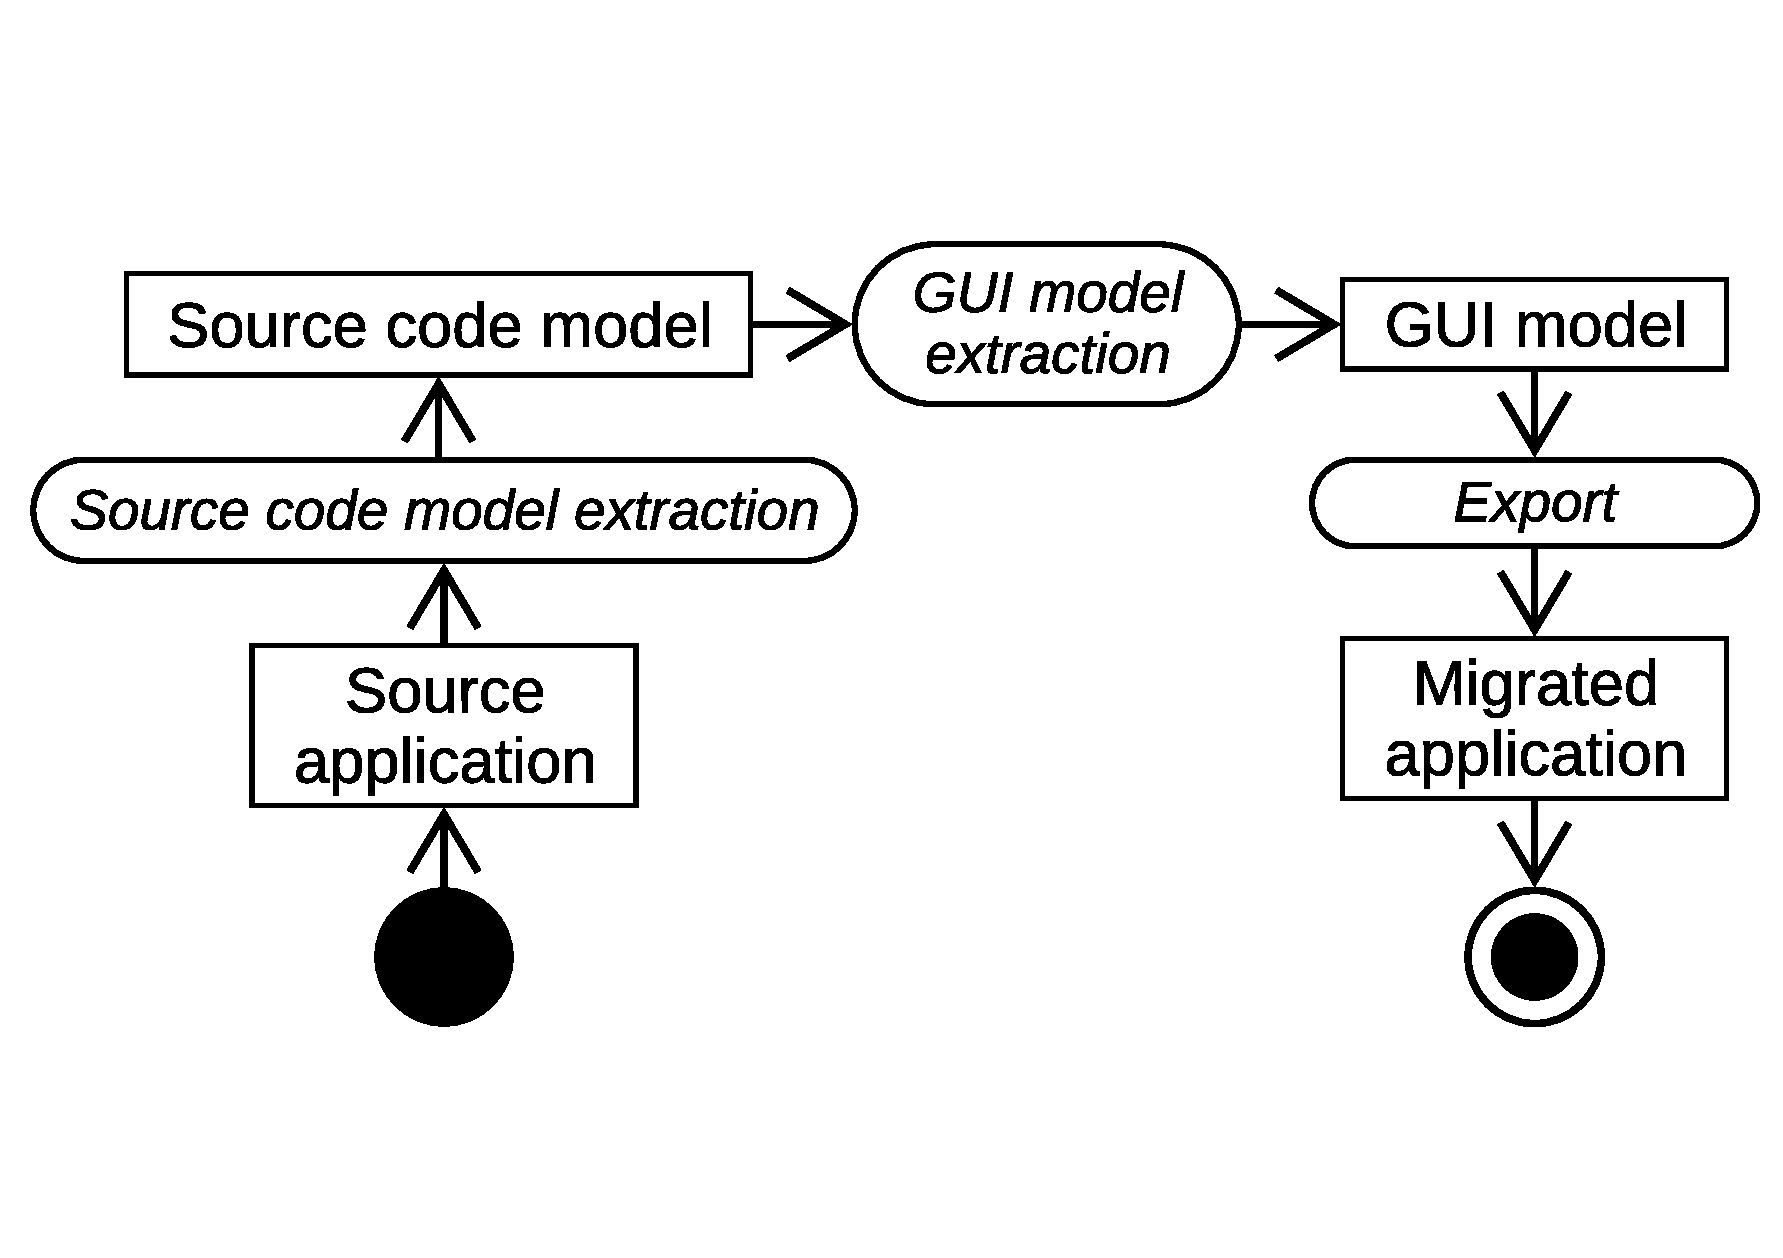
\includegraphics[width=0.6\linewidth]{processusMigration}
    \caption{Notre processus de migration}
    \label{fig:processusMigration}
    \end{center}
\end{figure}


Le processus, représenté \figref{processusMigration}, est divisé en trois étapes :

\begin{enumerate}
\def\labelenumi{\arabic{enumi}.}

\item \emph{Extraction du modèle du code source.} Nous construisons un modèle représentant le code source de l'application originale.
Dans notre étude de cas, le programme source est écrit en Java GWT.
L'extraction produit un modèle FAMIX \cite{Duca11c} de l'application utilisant un méta-modèle capturant les concepts Java.
Nous devons également analyser le fichier de configuration XML décrit dans la~\secref{comparisonGwtAngular}.

\item \emph{Extraction du modèle GUI.} 
Nous analysons le modèle de code source pour détecter les éléments du \emph{code visuel} décrivant l'interface graphique 
  et nous construisons un modèle d'interface graphique à partir de ces éléments. 
Le méta-modèle de l'interface graphique est décrit \secref{metamodelUI}.

% \item \em \emph{Extraction du code de comportement. } Une fois que le modèle d'interface graphique est
% généré, nous l'utilisons pour identifier les parties du modèle de code source correspondant à \emph{Behavioral code}.
% Par exemple, si un bouton est cliquable,
% the \emph{Code comportemental} est le code exécuté lorsqu'un utilisateur
% de clics sur le bouton.
% Ce \emph{Code comportemental} est lié à la représentation du bouton dans le modèle GUI.

\item \emph{Export.} Nous recréons l'interface graphique 
  % et le code de comportement 
  dans la langue cible.
Cette étape exporte les fichiers de l'interface utilisateur et 
les fichiers de configuration de l'application.

%\item \emph{Exportation du code comportemental. } Nous générons le \emph{Code comportemental} lié à l'interface utilisateur.
% Cette étape peut être effectuée en même temps que la précédente.
\end{enumerate}

Notez qu'actuellement nous ne traitons ni le \emph{code métier} ni le \emph{code comportemental} de l'application.
C'est sur ce point que porteront les travaux futurs.
  
\subsubsection{Méta-modèle GUI}
\label{sec:metamodelUI}

\begin{figure}[h]
  \begin{center}
  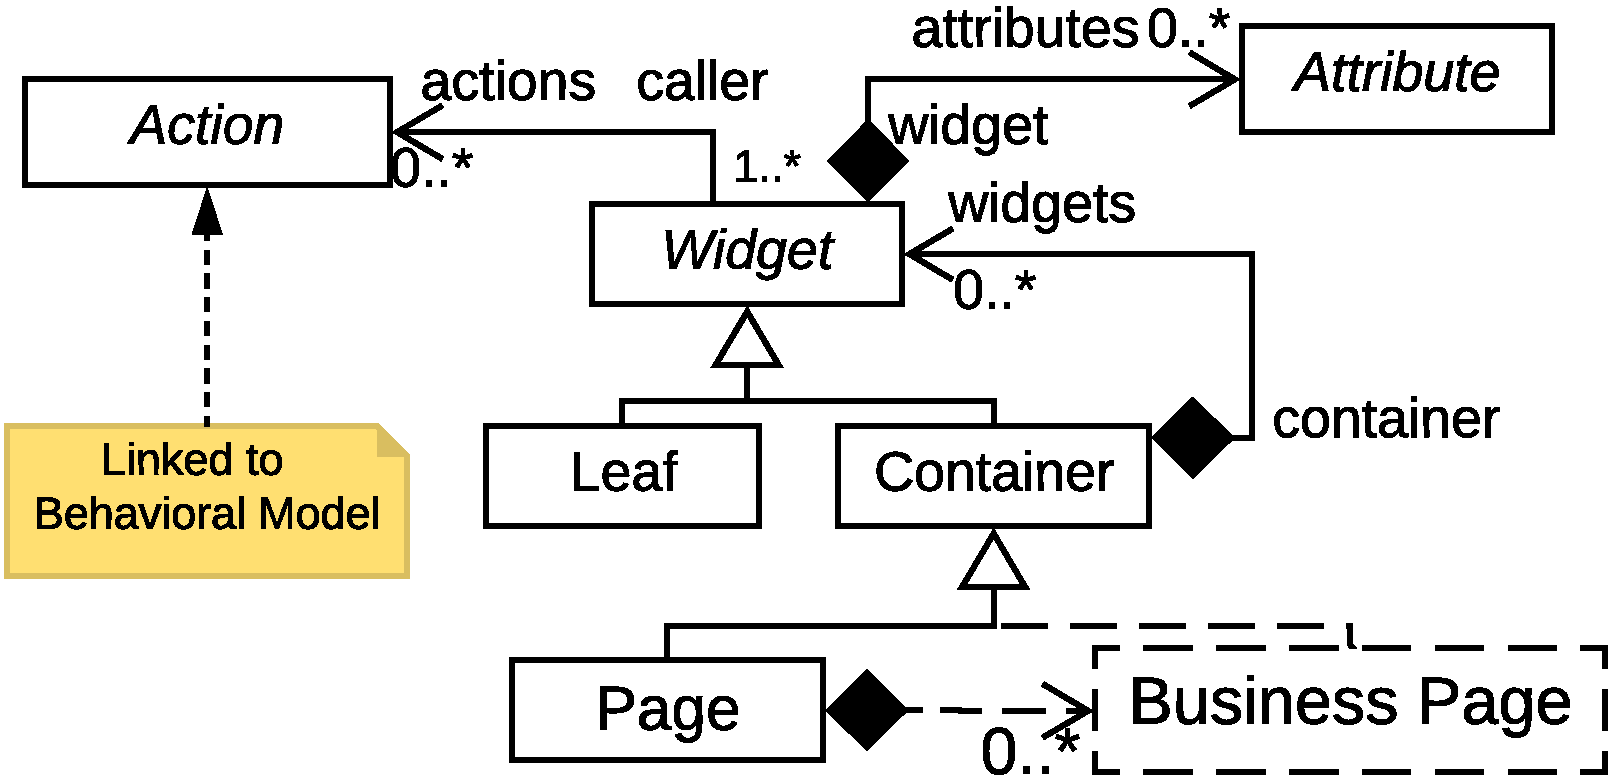
\includegraphics[width=0.5\linewidth]{GUIModel}
  \caption{Notre méta-modèle GUI}
  \label{fig:guimetamodel}
  \end{center}
\end{figure}
  
Afin de représenter les interfaces graphiques d'applications de bureau ou web, 
  nous avons conçu un méta-modèle GUI à partir de ceux présentés dans la~\secref{stateMetaUI}.
Le méta-modèle a été publié à SANER~2019 \citep{Verh19a}.
La~\figref{guimetamodel} représente notre méta-modèle.
Dans la suite de cette section, nous présentons les entités du méta-modèle.

% Représente les interfaces utilisateur d'applications de bureau ou web, 
% nous avons conçu un méta-modèle GUI présenté dans \figref{guiModel}.
% Ce méta-modèle est la synthèse des méta-modèles présentés dans \secref{stateMetaUI}. 
% Dans le reste de cette section, nous présentons les entités du méta-modèle.

% \picw{GUIModel}{Méta-modèle GUI}{fig:guiModel}{fig:guiModel}

Notre méta-modèle est une adaptation du méta-modèle KDM (voir \figref{kdm}).
Comme beaucoup d'autres, nous séparons les éléments graphiques correspondant au DOM des actions et événements.
Dans notre méta-modèle, les éléments graphiques sont appelés Widget. 
Ils peuvent être raffinés comme Leaf ou Container.

Dans notre contexte, l'interface graphique sera toujours affichée sur un écran.
Nous ne représentons donc pas tout le type d'UIDisplay et définissons une entité Page.
La Page représente le conteneur principal d'une interface graphique.
Cela peut être une fenêtre d'une application de bureau ou une page web.
La Page est un type de Container.

Comme proposé par de nombreux autres auteurs, nous avons ajouté l'entité Attribute dans notre méta-modèle d'interface graphique.
Un Attribute représente les informations d'un widget
  et peut changer son aspect visuel ou son comportement.
Quelques attributs communs sont la couleur ou la hauteur d'un widget. 
Il y a aussi des attributs qui contiennent des données.
Par exemple, un widget représentant un bouton peut avoir un attribut \emph{text} qui contient le texte du bouton.
Un attribut peut changer le comportement d'un widget, c'est le cas de l'attribut \textit{enable}.
Un bouton avec l'attribut \textit{enable} réglé sur \textit{false} représente un bouton sur lequel on ne peut pas cliquer.
Enfin, les widgets peuvent avoir des attributs qui ont un impact sur l'aspect visuel de l'application.
Ce type d'attribut permet de définir une mise en page à respecter par les widgets contenus dans le widget principal et peut
  éventuellement modifier les dimensions de ce dernier pour respecter une disposition particulière.

Ensuite, nous avons ajouté une entité Action.
Une Action représente une interaction entre un utilisateur et un widget.
Des types actions simples sont le clique ou le survole de la souris.
Une Action est reliée à un modèle comportemental qui sera le centre de nos travaux futur (voir~\secref{codeComportemental}). 

Finalement, la Business Page est une entité que nous avons dû ajouter pour mieux représenter leurs applications.
C'est un type de widget particulier défini dans le framework propriétaire BLCore de l'entreprise.

\subsubsection{Méta-modèle de layout}
\label{sec:layout}

Afin de représenter la disposition des widgets sur la page,
  nous avons conçus un méta-modèle représentant le layout, voir~\figref{layoutmetamodel}.
Nous avons soumis le travail sur les layouts à SCAM~2019\citep{Verh19e}.

\begin{figure}[h]
  \begin{center}
  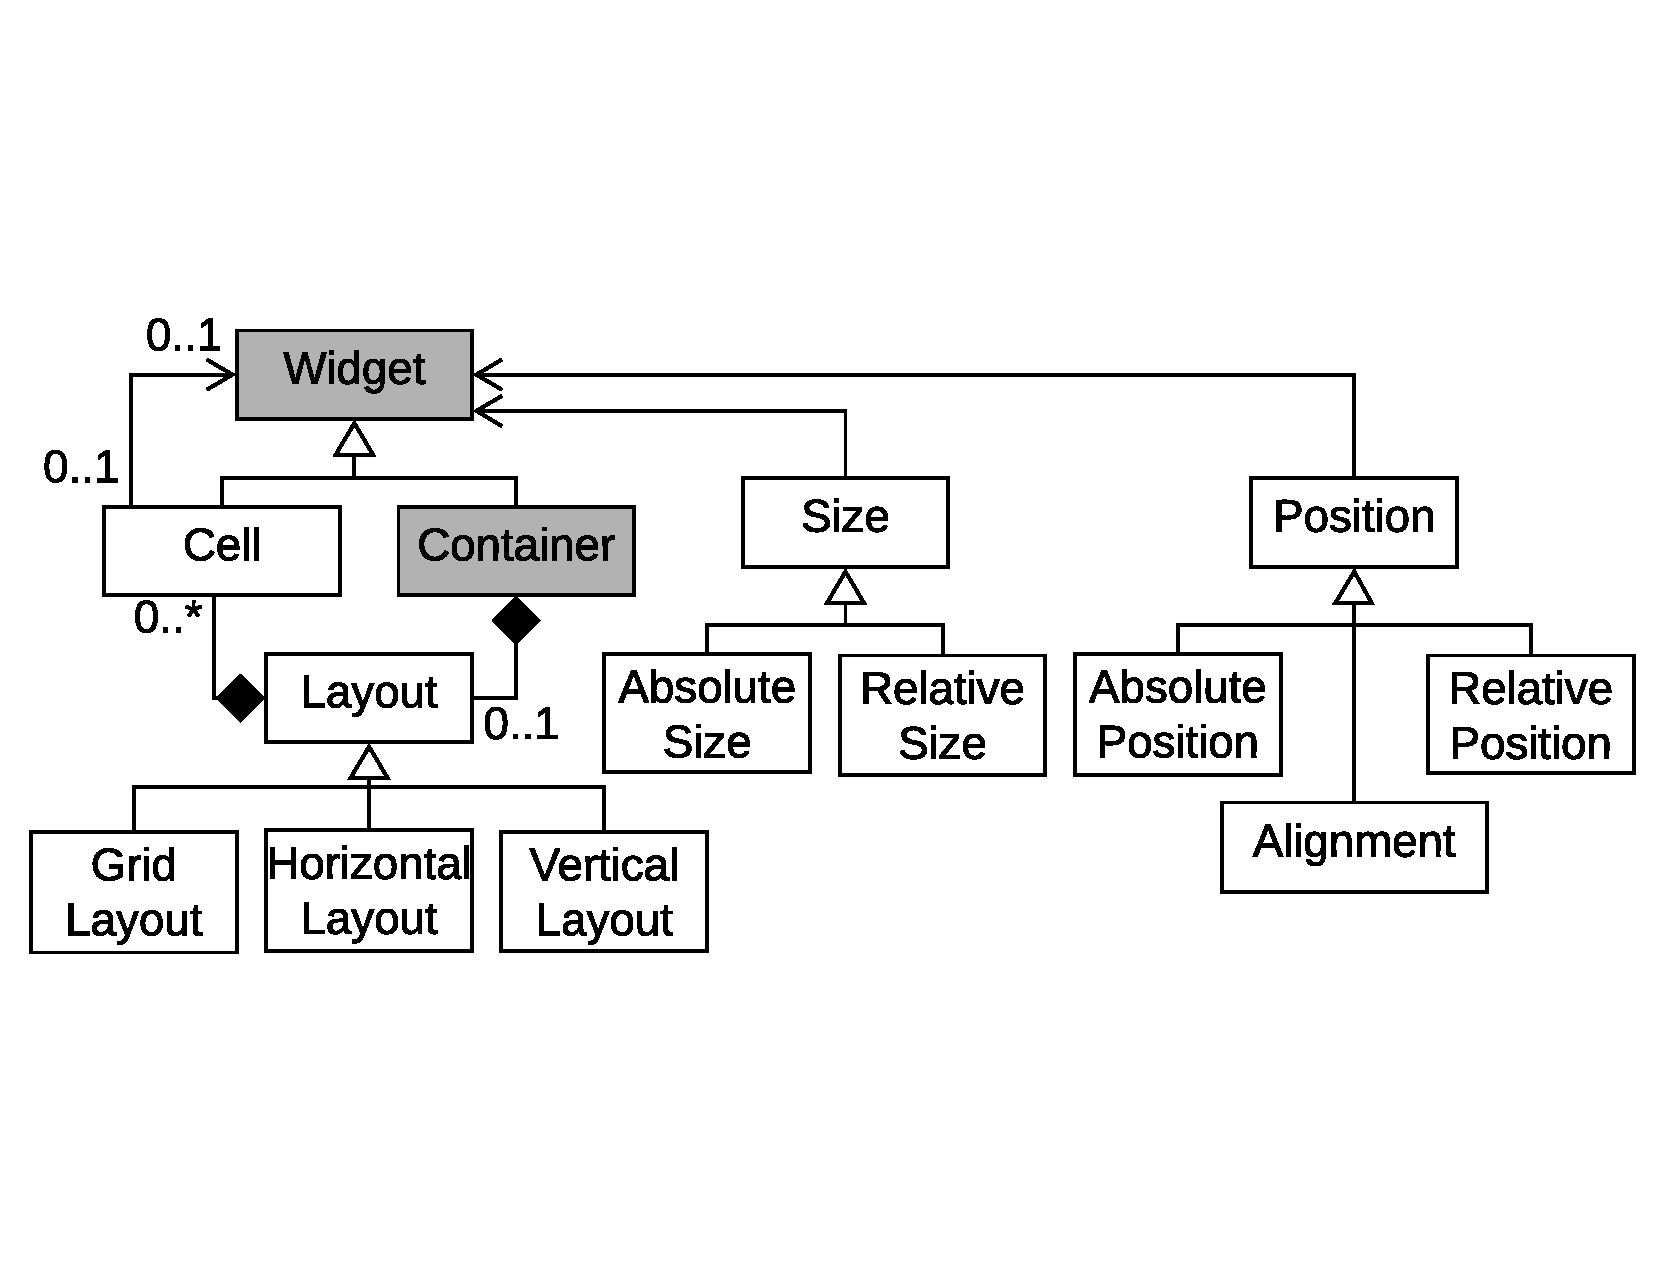
\includegraphics[width=0.7\linewidth]{layoutMetamodel}
  \caption{Notre méta-modèle de layout}
  \label{fig:layoutmetamodel}
  \end{center}
\end{figure}

Les entités Widget et Container font partie du méta-modèle GUI présenté \secref{metamodelUI}.

Le méta-modèle de layout ajoute trois entités principales au méta-modèle de l'interface graphique : 
    la Size ;
    la Position ; et
    le Layout.

L'entité Size décrit la hauteur et la largeur d'un widget.
La taille d'un widget peut être absolue ou relative.
Le AbsoluteSize représente une taille indépendante du conteneur du widget, exprimée en pixel.
Le RelativeSize représente la taille d'un widget par rapport à celle de son conteneur.
Elle est exprimée en pourcentage.

L'entité Position décrit la position d'un widget dans l'interface utilisateur.
Elle peut être absolue, relative ou définie grâce aux propriétés d'alignement.
Le AbsolutePosition représente la position du widget dans l'interface utilisateur.
Le RelativePosition représente la position d'un widget dans son conteneur.
L'Alignment définit comment placer le widget dans son conteneur.
Si le widget a une taille inférieure à son conteneur, il peut suivre les règles d'alignement.
Il peut être dans le \textit{haut}, \textit{bas}, \textit{droite}, \textit{gauche} or \textit{centre} 
    de son conteneur ou une combinaison de deux alignements, par exemple \textit{bas-droite}.

Le méta-modèle de layout ajoute l'entité Layout.
N'importe quel container du méta-modèle de l'interface graphique peut avoir un layout.
Le layout représente les règles pour disposer les enfants d'un container.
Un layout peut être affiné comme un Grid Layout ; un Horizontal Layout ou un Vertical Layout.
Il est possible d'adapter ce méta-modèle en ajoutant d'autres layouts.

Puisqu'un container a un layout, il ne contient plus directement de widgets.
Cela fait partie de la responsabilité du layout.
Un layout peut contenir plusieurs Cells.
Ces Cells contiennent les widgets du Container auxquelles elles appartiennent.

\subsection{Premier résultats}
\label{sec:resultats}

La~\secref{industrial} présente l'application sur laquelle nous avons validé notre approche.
La~\secref{retroImport} détaille les résultats de l'extraction des composants de l'application d'origine.
La~\secref{export} présente le résultat de l'exportation de l'application.
La~\secref{impact} présente les différentes propositions de collaborations que nous avons eu suite à la publication des travaux à Saner~19 \citep{Verh19a}.

\subsubsection{Application industrielle}
\label{sec:industrial}

Nous avons implémenté notre approche en Pharo puis l'avons expérimenté sur l'application \textit{kitchensink} de Berger-Levrault.
Notre outil est accessible et open-source\footnote{\url{https://github.com/badetitou/Casino}}.

Ce logiciel, dédié aux développeurs, a pour but de regrouper en une seule et même application l'ensemble des composants 
 disponible pour construire une interface graphique.
Cette application est plus petite qu'une application de production mais utilise le framework BLCore.
Le framework de l'entreprise nous garantit que le fonctionnement de l'application \textit{kitchensink} est
  exactement le même que les applications industrielles.
L'application contient 470 classes Java et représente 56 pages web.
Bien que ce soit l'application de démonstration pour les développeurs,
 l'application \textit{kitchensink} contient des irrégularités dans le code.

\subsubsection{Résultats de l'extraction}
\label{sec:retroImport}

La \tabref{resultImport} résume les résultats de l'extraction.

\begin{table}[htbp]
  \caption{Résultats de l'extraction}
  \vspace{-1.5em}
  \label{tab:resultImport}
  \begin {center}
    % \resizebox{\columnwidth}{!}{%
    \begin{tabular}{lcccc}
        \hline
          & \raisebox{-0.5em}{Pages} & \raisebox{-0.5em}{Business Pages} & Widgets \\
          &  &  & (sample) \\
        \hline
        \textbf{Nombre} & 56 & 76 & 238 \\
        \textbf{Correctement importé} & 100\% & 100\% & 89\% \\
        \hline
    \end{tabular} %
    % }
    \end{center}
\end{table}

L'outil a extrait 56 Pages de l'interface graphique originale.
Cela correspond au nombre de pages définies dans le fichier de configuration
  de l'application \textit{kitchensink}.

L'outil a extrait 76 Business Pages.
Cette valeur correspond exactement au nombre de business pages de l'application d'origine.
De plus, l'outil assigne correctement chaque Business Page à sa Page. 

Pour les widgets, nous avons analyser manuellement 6 pages de l'application d'origine
  ce qui représente un peu plus de 10\% des Pages de l'application.
Nous avons obtenu 100 \% des Widgets sur l'échantillon évalué qui ont été correctement détectés.
Cependant, 27 des 238 Widgets de notre échantillon (11\%) n'ont pas été correctement affectés à leur conteneur.
Tous ces problèmes viennent d'une seule et unique Page (contenant 75 Widgets au total).

\subsubsection{Résultats à l'exportation}
\label{sec:export}

Nous avons vérifié manuellement le nom des 56 pages exportées.
Elles conservent toutes leur nom d'origine.

\begin{figure}[htbp]
  \begin{subfigure}{0.49\textwidth}
    \fbox{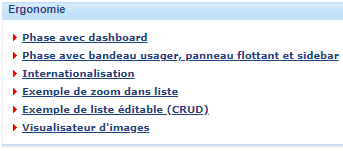
\includegraphics[width=0.9\linewidth]{cmp1/avant}}
    \caption{Page GWT original} 
    \label{fig:cmp1a}
  \end{subfigure}
  \hfill % separation between the sub-figures
  \begin{subfigure}{0.49\textwidth}
    \fbox{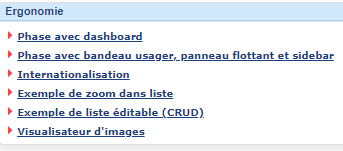
\includegraphics[width=0.9\linewidth]{cmp1/apres}}
    \caption{Page Angular après migration} 
    \label{fig:cmp1b}
  \end{subfigure}
  \caption{Comparaison du visuelle de la migration d'une Page} 
  \label{fig:cmp1}
\end{figure}

\begin{figure*}[hbtp]
  \begin{subfigure}{0.30\textwidth}
    \fbox{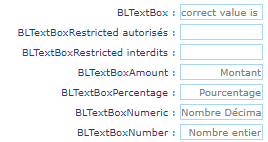
\includegraphics[width=0.9\linewidth]{cmp2/avant2}}
    \caption{Page GWT original} \label{fig:cmp2a}
  \end{subfigure}
  \hspace*{\fill} % separation between the sub-figures
  \begin{subfigure}{0.30\textwidth}
    \fbox{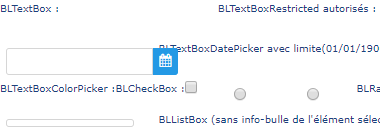
\includegraphics[width=0.9\linewidth]{cmp2/apres2}}
    \caption{Page Angular après migration sans modèle de layout} 
    \label{fig:cmp2b}
  \end{subfigure}
  \hspace*{\fill} % separation between the sub-figures
  \begin{subfigure}{0.30\textwidth}
    \fbox{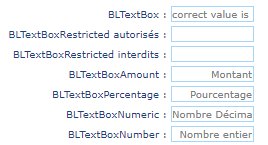
\includegraphics[width=0.9\linewidth]{cmp2/apresLayout2}}
    \caption{Page Angular après migration avec modèle de layout} 
    \label{fig:cmp2c}
  \end{subfigure}
  \caption{Comparaison du visuelle de la migration d'une Page avec et sans le méta-modèle de layout} 
  \label{fig:cmp2}
\end{figure*}

La~\figref{cmp1} présente les différences visuelles entre la version originale (GWT), à gauche, 
  et celle migrée (Angular 6), à droite.
On voit qu'il y a peu de différences. 
Dans la version exportée, la couleur de l'en-tête est un peu plus claire,
et les lignes sont un peu plus éloignées.

La~\figref{cmp2} présente les différences visuelles pour la Page \textit{Input box}. 
De nouveau sur le côté gauche il y a la Page original 
  au centre la même Page sans l'utilisation du modèle de layout
  et sur le côté droit la Page après la migration avec utilisation du modèle de layout. 
Comme les trois images sont grandes, nous les avons rognées pour afficher cette zone d'intérêt. 
Même si l'image du milieu est complètement différente, tous les widgets sont présents dans la version migrée.
Les différences visuelles sont dues à un problème dans la gestion de la mise en page.
La troisième image montre l'importance du modèle de layout dans la migration de l'interface graphique.
Avec le modèle de layout, la contrainte visuelle est satisfaite.

\subsubsection{Collaborations}
\label{sec:impact}

Suite à la publication de nos travaux à Saner~19 \citep{Verh19a}, plusieurs entreprises se sont intéressées à nos travaux.

Tout d'abord, au vu des résultats que nous avons obtenus, 
  Berger-Levrault a décidé d'expérimenter nos travaux sur plusieurs sujets de migration:
  la migration d'applications Silverlight vers Aurelia et la migration d'applications AngularJS vers Angular\footnote{Malgré une ressemblance dans le nom, les frameworks AngularJS et Angular ont de nombreuses différences}.
Dans la continuité de ce travail, Berger-Levrault a décidé d'initier une autre thèse qui sera le prolongement de celle-ci.

En plus de Berger-Levrault, trois entreprises nous ont contactés pour travailler sur la problématique de migration d'interface graphique.
La première, AKIO, cherche actuellement une solution pour migrer ses applications de GWT vers Angular.
La deuxième, parcIT, une entreprise allemande, désire migrer ses applications GWT en View.js.
Enfin, la troisième, Orange Business Service veut travailler avec nous à partir de décembre pour la migration de leurs applications GWT vers Angular.

\section{Roadmap}
\label{sec:roadmap}

Cette section présente les différents travaux sur lesquels nous souhaitons travailler pour la suite de cette thèse.
% La~\secref{layout} expose le travail qui a été fait et restant pour un meilleur support des layouts.
La~\secref{migrationMultiLangage} présente le travail sur le support de multiples langages.
La~\secref{codeComportemental} discute de la migration du code comportemental.
La~\secref{codeMetier} expose le travail nécessaire pour migrer le code métier.
La~\secref{validationAutomatique} présente le travail à réaliser pour valider automatiquement tout ou parti de la migration d'une application.
% La~\secref{composants} détaille une étape permettant d'améliorer le résultat des migrations utilisant des frameworks propriétaire.
% La~\secref{industrialisation} présente l'industrialisation de notre travail à Berger-Leavrault.
Enfin, la~\secref{redaction} présente les dates utilisées pour la rédaction du sujet de thèse.

La~\figref{chronologie} représente la roadmap actuelle.

\begin{figure}[h]
  \begin{center}
  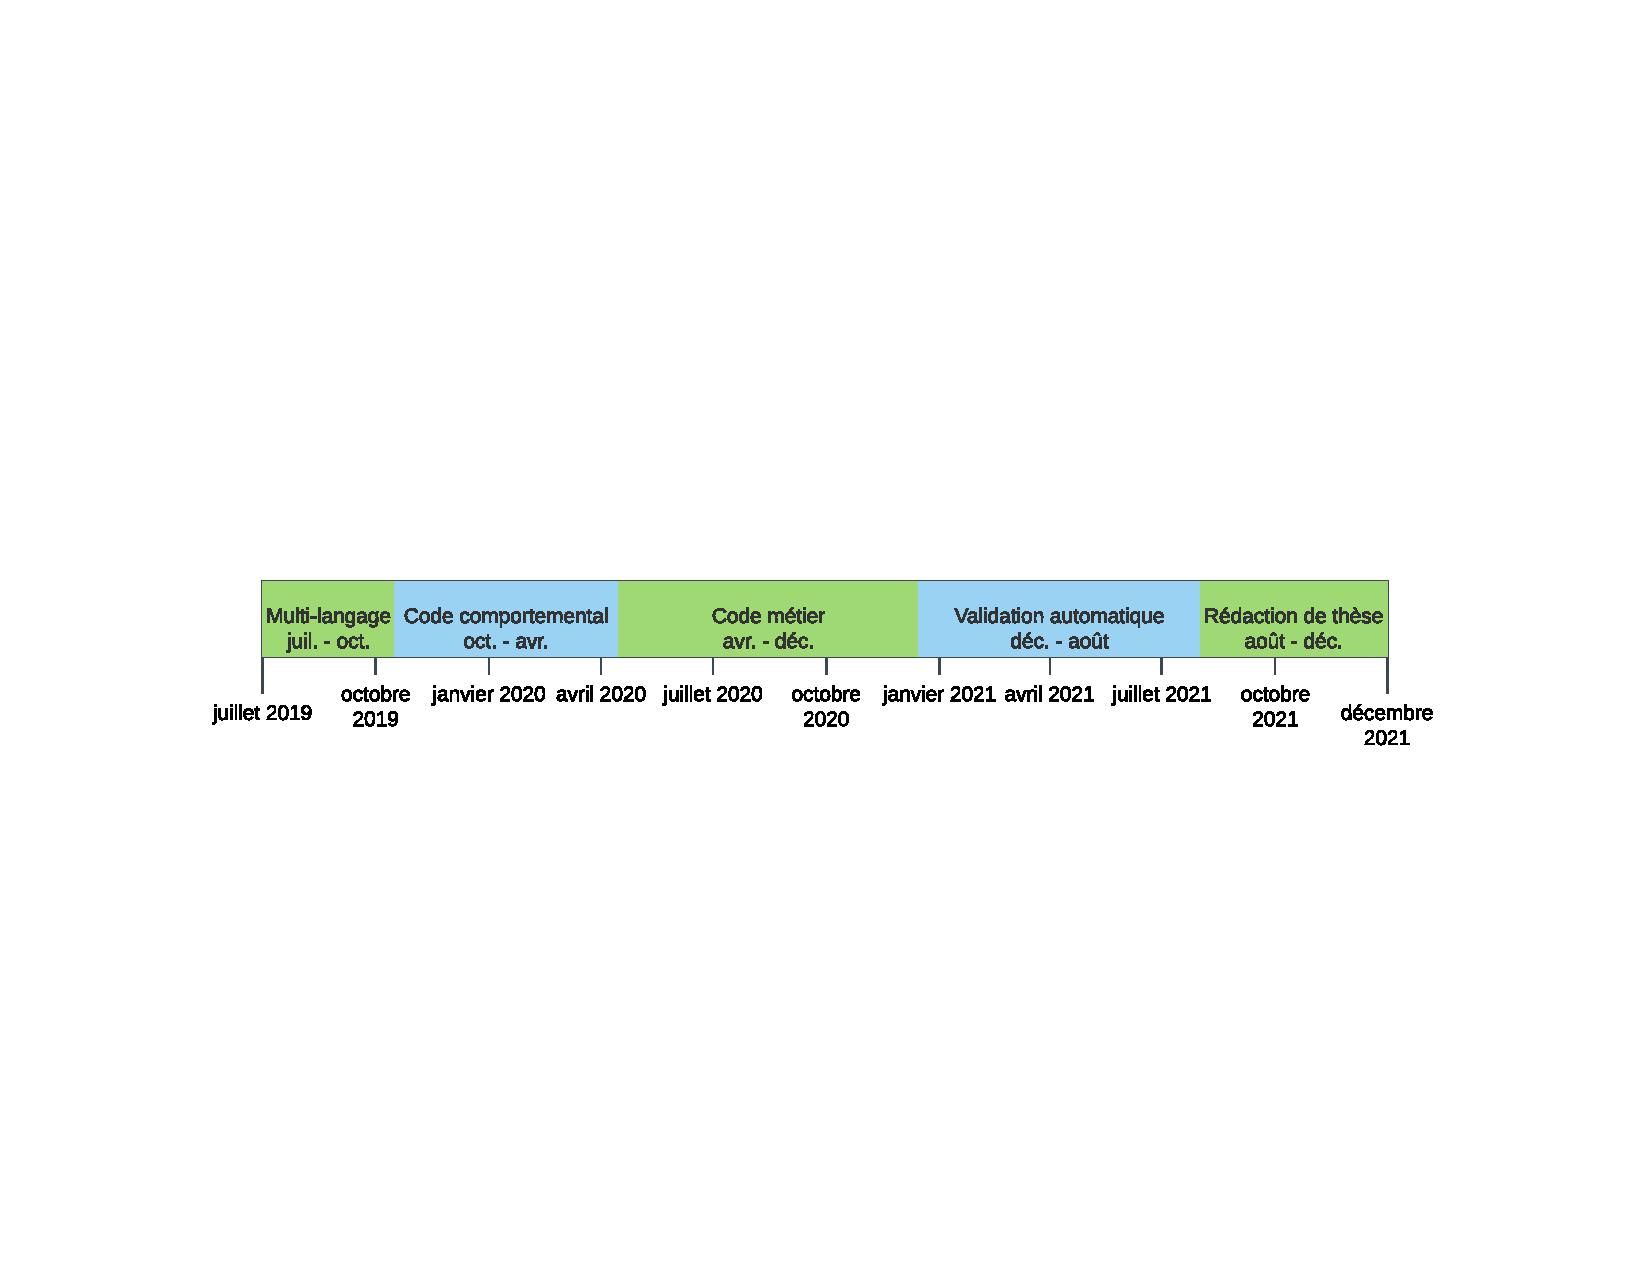
\includegraphics[width=1\linewidth]{Chronologie}
  \caption{Chronologie prévisionnel de la suite de la thèse}
  \label{fig:chronologie}
  \end{center}
\end{figure}

\subsection{Migration Multi-Langage}
\label{sec:migrationMultiLangage}

Afin de valider que notre méta-modèle d'interface graphique et notre approche sont génériques,
  nous avons prévu de travailler sur la migration d'applications avec d'autres langages source et cible.
Il s'agit de la prochaine étape de notre travail.

Afin d'accomplir cet objectif, nous avons déjà mené des travaux préliminaires en migrant des applications de Spec\footnote{Spec est un framework permettant la conception d'interface graphique en Pharo} vers Spec~2.
Ces travaux ont été présenté dans un papier soumis à IWST \citep{Verh19d}.
En même temps, Berger-Levrault souhaite utiliser notre solution dans d'autres cas de migration comme celle de Silverlight vers Aurelia.
Enfin, plusieurs autres entreprises nous ont contactés afin d'étudier la possibilité d'utiliser notre approche sur d'autres cas de migration, par exemple de GWT vers view.js.

Ce sujet devrait être le centre de nos recherches jusqu'au mois d'octobre 2019
  et nous désirons rédiger un article de journal sur ce travail.

\subsection{Code comportemental}
\label{sec:codeComportemental}

Lors de notre décomposition d'une interface graphique, 
  nous avons identifié le code comportemental comme représentant le code exécuté lorsqu'un utilisateur réagit avec l'interface.
Afin de migrer ce code, nous allons devoir l'identifier, l'extraire et l'exporter dans le langage cible.

Une première idée, qui permettrait de continuer avec l'approche que nous avons mise au point
  serait d'utiliser un modèle pivot de code comportemental.
Afin d'améliorer les résultats de la migration,
  le meta-modèle de code comportemental pourrait être composé d'entités spécifiques au domaine des interfaces graphiques.
Pour représenter les structures de contrôle, \ie boucles, alternatives, ce meta-modèle pourrait ce baser sur un méta-modèle représentant un AST.

Une fois le travail sur la migration multi-langage terminé,
  le support du code comportemental sera notre travail principal.
Nous planifions de travailler sur ce sujet jusqu'au mois de février 2020 afin de soumettre un papier en avril 2020 à ICSME.

\subsection{Code métier}
\label{sec:codeMetier}

En plus de migrer les composants de l'interface graphique, partie visuelle, 
  et le comportement de l'interface lors des interactions utilisateurs, code comportemental,
  nous voulons migrer les règles de l'application et les données qu'elle utilise.
Par exemple, les applications de Berger-Levrault sont composées de nombreux tableaux.
Ce widget, bien que simple en apparence, utilise de nombreuses fonctionnalités du framework d'Interface Graphique.
En particulier l'adaptation aux données qu'il doit afficher
  et la gestion des habilitations de l'utilisateur.

Afin de s'adapter aux données à afficher, il faut en extraire la structure.
Cette extraction fait parti de la migration du code métier.
Lors de l'exportation vers le langage cible, 
  le code métier sera traduit dans la création des structures de données manipulées 
  et du code pour manipuler ces données.

Pour la gestion des habilitations, 
  les applications de Berger-Levrault sont utilisées par différents utilisateurs au sein d'une même organisation.
Ces utilisateurs non pas forcément les mêmes droits d'accès aux données, \eg lecture, écriture, aucun.
Les droits d'accès proviennent de règles définies pour une application 
  et impactent l'interface graphique.
Il est donc essentiel d'extraire les habilitations et de les traduire dans le code de l'application migrée.
Cette règle de gestion fait partie du code métier.

Enfin de migrer correctement tous le code métier, 
  il sera intéressant d'étudiant l'extraction des règles métier depuis l'application originale.

Nous n'avons pas encore trouvé de travaux relatifs à ce sujet.
Une fois cette étape finie, l'objectif est de pouvoir migrer correctement une application 
  avec son aspect visuel, son comportement et les interactions avec le back-end.

Nous devrions faire ce travail de mai 2020 à décembre 2020.

En plus de cette thèse, une seconde thèse est menée à Berger-Levrault 
  sur la migration du back-end des applications.
En fonction de l'avancement de cette seconde thèse, 
  nous pourrions profiter de ce temps pour travailler ensemble 
  et essayer d'améliorer les résultats de la migration de chacun des travaux.

\subsection{Validation automatique}
\label{sec:validationAutomatique}

La validation automatique de la migration est actuellement un problème non résolu.
Elle est nécessaire pour la validation du code visuel, comportemental et métier.
Il est possible de vérifier manuellement le résultat de la migration pour quelques pages 
  mais il est préférable de le faire automatiquement pour des centaines de pages (plus de 400 sur les applications de Berger-Levrault).

Nous n'avons trouvé, dans la littérature, que peu d'approches envisageant une validation visuelle automatique.
Dans deux articles \citep{Sanc14a,Joor12a}, les auteurs comptent simplement le nombre de widgets dans les applications sources et les applications cibles.
Mais nous avons vu dans \figref{cmp2} que cela ne garantit pas la similarité visuelle.
Un autre article \citep{Mora18a} propose de comparer les captures d'écran de l'application originelle et de l'application exportée pixel par pixel.
Cependant, nous avons vu \figref{cmp1} que des écrans aux différences à peine distinguables peuvent avoir des différences au niveau des pixels.
Enfin, d'autres travaux portent sur la recherche de similarité de layout entre deux documents \citep{Cao10a,Hu99a,Egli03a}.
Ces travaux peuvent nous aider à détecter des erreurs de layout entre des pages mais ne détecteront pas les erreurs dans le contenu des pages ou dans leurs comportements. 


Une solution serait pour valider la migration serait d'utiliser les tests de l'application originelle.
Cependant, dans le cas des applications de Berger-Levrault, il n'y a pas de tests développés pour l'interface graphique.
Nous ne pouvons donc pas les utiliser pour notre cas d'étude.
Il faudrait alors générer les tests vérifiant le comportement de l'interface.
Ces tests peuvent être créés à partir des comportements détectés lors de l'extraction du code visuel et comportemental ou
   à partir de cas de test définis manuellement par l'entreprise.
 Ce dernier est déjà à l'étude pour d'autres projets par le service recherche de Berger-Levrault.

Ce travail devrait être effectué du mois de janvier 2021 au mois d'août 2021.

% \subsection{Migration des composants}
% \label{sec:composants}

% Notre stratégie de migration se base sur les widgets déjà préexistants dans le framework source et le framework cible.
% Bien que les widgets simples sont très souvent présents dans tous les frameworks d'interface graphique, \eg les boutons, les tableaux,
%   certains composants plus complexes présents dans le framework source ne trouvent pas d'équivalents dans le framework cible.

% Il peut exister deux raisons à cela.
% Le composant dans l'application source n'est pas un composant standard dans le framework cible, 
%     les applications de bureau ont, par exemple, souvent des toolbar contrairement aux applications web.
% Le composant dans l'application source est spécifique à l'application elle-même ou fait partie d'un kit de développement propre à l'entreprise qui l'utilise, 
%   ce sont des composants propriétaires.

% Dans chacun des cas, 
%   le composant complexe peut avoir été créé à partir d'une couche graphique de bas niveau, par exemple un canvas sur lequel sont dessinées des formes,
%   ou grâces à une composition de composant plus simple avec des règles spécifiques.
% Pour ce dernier cas, il serait alors possible d'extraire la structure d'un composant complexe.
% En découvrant les composants complexes utilisés dans une application front-end,
%   et en extrayant les informations de ces derniers il sera alors possible d'ajouter des widgets à notre approche depuis l'application à migrer,
%   et de migrer les composants complexes dans le framework cible.

% Nous pensons effectuer ce travail du mois de janvier 2021 au mois de avril 2021.

% \subsection{Industrialisation}
% \label{sec:industrialisation}

% Du mois de mai 2021 à juillet 2021, nous avons prévu de nous concentrer sur l'industrialisation
%   de notre travail afin de faire de ce projet de thèse un succès industriel.

% Cette industrialisation passe par l'utilisation de notre approche sur l'ensemble des applications utilisant
%   GWT dans l'entreprise.
% Puisque les développeurs souhaitent pouvoir migrer les applications en continu, c'est à dire en faisant fonctionner
%   en parallèle la version GWT et la version Angular, nous allons mettre en place des outils leur permettant ce cas d'utilisation.

% Durant cette phase, il sera intéressant de regarder si notre outil peut apprendre des corrections faîtes par les développeurs.
% Par exemple, un développeur détecte une erreur qui apparaît régulièrement, 
%   il pourrait alors interagir sur l'outil de migration pour mieux orienter la migration des futurs interfaces.

\subsection{Rédaction de thèse}
\label{sec:redaction}

Enfin les mois d'août 2021 à décembre 2021 seront utilisés pour la rédaction de la thèse 
  et les derniers ajustements des objectifs décrits ci-dessus.


\section{Publications}

Cette section présente la liste des publications et soumissions liée à cette thèse.

\subsection{Papiers publiés}

\begin{enumerate}
  \item Conférence internationale : \bibentry{Verh19a}
  \item Conférence nationale : \bibentry{Verh19b}
  \item Workshop internationale : \bibentry{Verh19c}
\end{enumerate}

\subsection{Papiers soumis}

\begin{enumerate}
  \item Workshop internationale : \bibentry{Verh19d}
  \item Conférence internationale de rang C : \bibentry{Verh19e}
\end{enumerate}

\section{Formation doctorale}

Je n'ai pas encore participé à des formations de l'école doctorale car mon inscription c'est faîte en Janvier et j'ai obtenu les code d'accès au site des formations en Mars 
  et les dernières formations ont eu lieu alors que j'étais en déplacement pour des conférences ou en déplacement à Berger-Levrault à Montpellier.

Cependant, je participe à une école d'été du 11 au 12 Juillet 2019.

Je fais ma thèse à moitié depuis Montpellier là où se situe les équipes de Berger-Levrault pour qui je travaille. Du coup, il est un peu compliqué pour moi de suivre les formations. 
Je pense m'inscrire dès que les inscriptions seront ouvertes sur des formations en particulier en enseignement et l'éthique scientifique. 
Je suivrai aussi des tutoriels lors de conférence dans la mesure des possibilités.

\section{Projet professionnel}

A la suite de la thèse, je souhaite continuer à travailler dans la recherche dans le milieu académique.
Pour cela, je prévois d'effectuer un post-doctorat à l'étranger.
J'aimerais pouvoir poursuivre dans l'étude de l'évolution des logiciels et comment l'améliorer et la simplifier.
Ceci fait écho avec ce projet de thèse sur l'évolution des applications ayant une interface graphique
  ainsi qu'avec d'autres travaux que j'ai fait sur l'utilisation des tests \citep{Verh17a, Deme18a}.

L'objectif final est de pouvoir continuer la recherche dans une université,
  et d'encadrer des étudiants sur des projets de recherche (doctorant) ou non (stagiaire de l'université par exemple).
Dans cette optique, j'ai déjà commencé à encadrer des étudiants au sein de mon entreprise 
  et j'ai travaillé avec un étudiant au laboratoire de l'Inria, ce qui a conclu à la soumission d'un papier de recherche pour IWST 2019.
Et j'enseigne à Polytech Lille en première et deuxième année du cycle ingénieur, 46 heures en 2018/2019 et 36 heures en 2019/2020,
  ainsi qu'en master 2 et en licence 2 à l'université de Montpellier, 4 heures en 2018/2019 et 30 heures en 2019/2020. 


\footnotesize{
  %\bibliographystyle{alpha}
  % natbib 
  %\bibliographystyle{myplainnat}
  \bibliographystyle{mySmallPlainnat}
  \bibliography{others,rmod,nextPubli}
}

\end{document}